%\documentclass[a4paper, 12pt]{report}
\documentclass[12pt,a4paper,openany]{abntex2}

\usepackage[T1]{fontenc}
%\usepackage[latin1]{inputenc}
%\usepackage[verbose,left=30mm,right=20mm,top=30mm,bottom=30mm]{geometry}
%\usepackage{txfonts}
\usepackage[brazil]{babel}
\usepackage{pdfpages}
%\usepackage[authoryear]{natbib}
%\usepackage{appendix}
%\usepackage{setspace}
%\usepackage{url}
%\usepackage{hyperref}
%\usepackage{color}
\usepackage[utf8]{inputenc}
\usepackage{placeins}
\usepackage{float}

\autor{Leonardo Mendonça de Araujo \and \\ Lucas Bagatini do Nascimento \and \\ Mário Muramatsu Júnior}
\titulo{RELATÓRIO DE FINAL: IDENTIFICADOR DE SINAIS TRIFÁSICOS}
\data{2018} 
\local{Rio Claro, São Paulo}
\preambulo{Monografia apresentada ao curso de Ciências da Computação, como requisito parcial para a obtenção do Título de Bacharel em Ciências da Computação, Instituto de Geociências e Ciências Exatas da Universidade Estadual Paulista}
\orientador{Mario Roberto da Silva}
\tipotrabalho{monografia}

\begin{document}
	
\imprimircapa	
\imprimirfolhaderosto

\clearpage
\cleardoublepage
\cleardoublepage

\pagenumbering{arabic}
\setcounter{page}{3}

\tableofcontents
\clearpage{\pagestyle{empty}\cleardoublepage}
	
\chapter{Introdução}

\section{NOME DA SEÇÃO}

%----------------Exemplo: insere figura-----------------------
%\begin{figure}[!htp]
%	\centering
%	\fbox{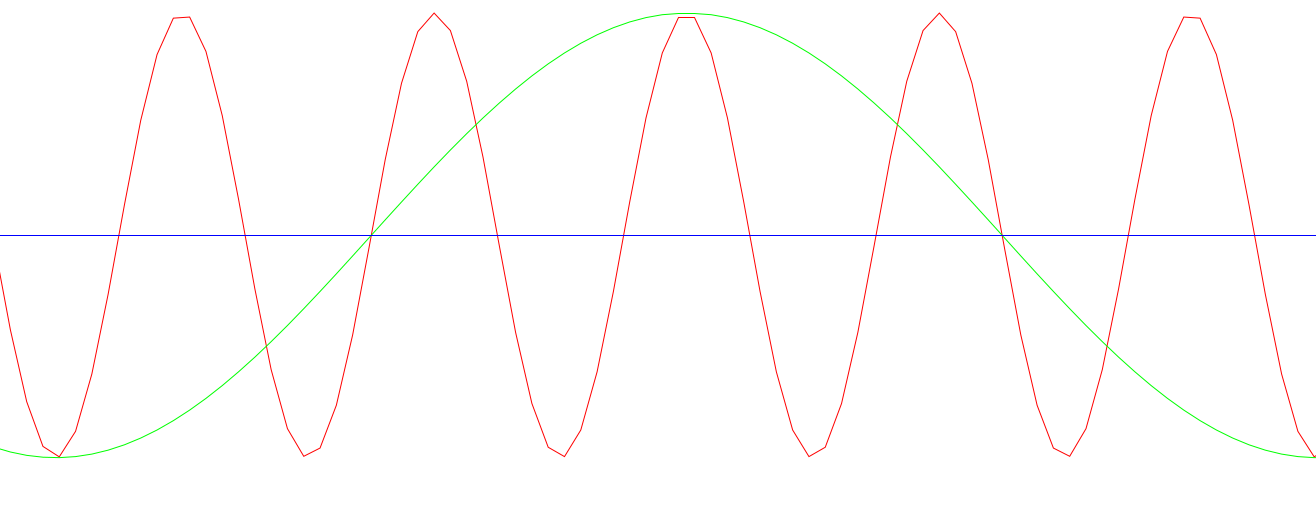
\includegraphics[width=16cm]{images/ondas.png}}
%		\caption{Exemplo de ondas sonoras}
%	\label{fig:ondas-sonoras}
%\end{figure}

%---------------Exemplo: insere tabela -----------------------
%\begin{table}[h]	
%	\centering	
%	\vspace{0.5cm}	
%\begin{tabular}{r|lr}
%Notas  & Frequ{\^e}ncia (Hz) \\
%\hline 
%C (Dó) & 261,33          \\
%D (Ré) & 293,66          \\
%E (Mi)  & 329,63 		 \\
%F (Fá)  & 349,23 		 \\
%G (Sol) & 391,99 		 \\  
%A (Lá)  & 440,00  		 \\
%B (Si)  & 493,88
%\end{tabular}
%	\label{tab:frequencia-notas}
%	\caption{Frequência da notas centrais do piano}
%\end{table}

\end{document}
